\documentclass[12pt,a4paper]{article}

% ─── Packages ───
\usepackage[utf8]{inputenc}
\usepackage[T1]{fontenc}
\usepackage{mathptmx}           % Times font
\usepackage{amsmath,amssymb}
\usepackage{graphicx}
\usepackage[margin=1in]{geometry}
\usepackage{booktabs}
\usepackage{hyperref}
\usepackage{natbib}
\usepackage{caption}
\usepackage{float}
\usepackage{setspace}
\onehalfspacing

\hypersetup{
    colorlinks=true,
    linkcolor=blue!60!black,
    citecolor=blue!60!black,
    urlcolor=blue!60!black,
}

% ─── Title ───
\title{\textbf{Statistical Isomorphism Between Phanerozoic Tectonic Rhythms \\
and Riemann Zeta Zero Spacings: \\
A Random Matrix Theory Perspective}}

\author{
    Ruqing Chen \\
    \textit{GUT Geoservice Inc., Montreal, Canada} \\
    \texttt{ruqing@hotmail.com}
}

\date{June 2026}

\begin{document}

\maketitle

% ─── Abstract ───
\begin{abstract}
We investigate whether the temporal spacing of major geological boundaries in the Phanerozoic eon (538.8\,Ma to present) exhibits statistical signatures characteristic of random matrix ensembles, specifically the Gaussian Unitary Ensemble (GUE) and Gaussian Orthogonal Ensemble (GOE), or whether it follows a Poisson (memoryless) process. Using all 102 ICS 2023-standard stage-level boundaries, we extract 99 inter-event intervals and compare their normalized spacing distribution against the Wigner surmise for GUE ($\beta=2$), GOE ($\beta=1$), and Poisson statistics via Kolmogorov--Smirnov tests, Anderson--Darling statistics, nearest-neighbor spacing ratios, higher-moment analysis, and bootstrap confidence intervals. We find that (1)~the Poisson hypothesis is decisively rejected at $p = 1.3 \times 10^{-4}$ and with an $11.6\sigma$ deviation in the spacing ratio statistic; (2)~the GOE model provides the best overall fit across all test statistics (KS $D = 0.090$, $p = 0.38$; $A^2 = 1.18$); and (3)~the GUE model, while close in spacing ratio ($\langle r \rangle = 0.637$, only $1.6\sigma$ from GUE theory), is marginally rejected by higher-order tests. As a methodological control, we verify that the first 500 non-trivial zeros of the Riemann zeta function conform precisely to GUE statistics. We conclude that Earth's tectonic system displays clear level repulsion in its event timing---characteristic of a correlated dynamical system---at the GOE ($\beta \approx 1$) universality class, intermediate between Poisson randomness and the full GUE repulsion seen in the Riemann spectrum.

\medskip
\noindent\textbf{Keywords:} random matrix theory; Phanerozoic; geological boundaries; level repulsion; Riemann zeta function; GUE; GOE; Wigner surmise; tectonic rhythms; mass extinctions

\medskip
\noindent\textbf{Code and data:} \url{https://github.com/Ruqing1963/geo-riemann-spectral-statistics}
\end{abstract}


% ═══════════════════════════════════════════════════
\section{Introduction}
% ═══════════════════════════════════════════════════

The Phanerozoic eon, spanning the last 538.8 million years, represents the period of Earth's history during which complex multicellular life has existed. This interval is punctuated by a sequence of major geological boundaries---period, epoch, and age-level transitions defined by the International Commission on Stratigraphy (ICS)---as well as at least five catastrophic mass extinction events. A fundamental question in geodynamics is whether the temporal spacing of these events is essentially random (a Poisson process), or whether the Earth system exhibits correlated timing behavior in which events are not independent but exhibit some form of mutual interaction.

Independently, in number theory and mathematical physics, the non-trivial zeros of the Riemann zeta function have been shown to exhibit remarkable statistical properties. Montgomery~\citep{montgomery1973} conjectured, and Odlyzko~\citep{odlyzko1987} numerically demonstrated, that the normalized spacing distribution of Riemann zeros follows the statistics of the Gaussian Unitary Ensemble (GUE) of random matrix theory---the same statistics governing energy level spacings in quantum systems with broken time-reversal symmetry. This GUE behavior is characterized by \emph{level repulsion}: zeros (or energy levels) tend to avoid clustering, producing a spacing distribution with a characteristic suppression near zero.

The universality of random matrix statistics across disparate physical systems---nuclear spectra, quantum billiards, zeros of $L$-functions---invites the question of whether macroscopic geophysical systems might also belong to a random matrix universality class. Previous work has explored connections between random matrix theory and seismicity~\citep{telesca2011}, climate records, and astrophysical timing. The question of periodicity in geological extinctions was famously raised by Raup and Sepkoski~\citep{raup1984}, though the strict periodicity hypothesis has remained controversial. Here, we adopt a different approach: rather than testing for periodicity, we ask whether the \emph{statistical distribution} of inter-event spacings conforms to a random matrix ensemble, and if so, which one.

We test three competing models: (1)~the Poisson distribution, corresponding to independent, memoryless events; (2)~the GOE Wigner surmise ($\beta = 1$), representing systems with weak level repulsion and time-reversal symmetry; and (3)~the GUE Wigner surmise ($\beta = 2$), representing maximal repulsion with broken time-reversal symmetry, as seen in Riemann zeros.


% ═══════════════════════════════════════════════════
\section{Data and Methods}
% ═══════════════════════════════════════════════════

\subsection{Geological Boundary Ages}

We adopt the complete set of Phanerozoic age/stage-level boundaries from the International Chronostratigraphic Chart \citep[ICS, version 2023/09;][]{cohen2023}. This includes 102 stage boundaries spanning from the Fortunian (base of the Cambrian, 538.8\,Ma) to the Meghalayan (0.0042\,Ma). After filtering sub-Holocene microintervals ($\Delta T < 0.1$\,Ma) which reflect climatostratigraphic rather than tectonic signals, we retain $n = 99$ inter-boundary intervals with a mean spacing of $\langle\Delta T\rangle = 5.44$\,Ma and standard deviation $\sigma = 3.54$\,Ma.

This represents a substantial improvement in statistical power over period-level analyses (which yield only ${\sim}12$ intervals), placing our sample size in a regime where distributional tests carry meaningful discriminatory power. The complete dataset is available in the repository at \texttt{data/ics2023\_stages.csv}.

\subsection{Riemann Zeta Zeros (Control Dataset)}

As a methodological control, we compute the first 500 non-trivial zeros of the Riemann zeta function $\zeta(s)$ using the \texttt{mpmath} library at 15-digit precision. The imaginary parts $\gamma_n$ are extracted and their spacings normalized using the standard asymptotic density function
\begin{equation}
    \rho(\gamma) = \frac{1}{2\pi} \log\frac{\gamma}{2\pi},
\end{equation}
yielding a sequence $\delta_n = (\gamma_{n+1} - \gamma_n) \cdot \rho(\gamma_n)$ with unit mean. This dataset provides a known GUE-distributed reference against which our methods can be validated.

\subsection{Normalization and Theoretical Distributions}

The geological intervals $\Delta T_i$ are normalized by their sample mean to produce a dimensionless spacing sequence $s_i = \Delta T_i / \langle\Delta T\rangle$ with unit mean. We compare the empirical distribution against three theoretical models:
\begin{align}
    p_{\text{GUE}}(s) &= \frac{32}{\pi^2}\, s^2\, \exp\!\left(-\frac{4s^2}{\pi}\right), \label{eq:gue} \\[4pt]
    p_{\text{GOE}}(s) &= \frac{\pi}{2}\, s\, \exp\!\left(-\frac{\pi s^2}{4}\right), \label{eq:goe} \\[4pt]
    p_{\text{Poisson}}(s) &= e^{-s}. \label{eq:poisson}
\end{align}
The GUE and GOE distributions both exhibit level repulsion ($p(s) \to 0$ as $s \to 0$), with GUE showing stronger quadratic suppression compared to GOE's linear suppression. The Poisson distribution has maximal probability at zero spacing, reflecting the absence of inter-event correlations.

\subsection{Statistical Tests}

We employ the following suite of complementary diagnostics:

\paragraph{Kolmogorov--Smirnov (KS) test.} Measures the maximum absolute difference $D = \sup_s |F_n(s) - F(s)|$ between the empirical CDF $F_n$ and each theoretical CDF $F$. The associated $p$-value tests the null hypothesis that the data are drawn from the specified distribution.

\paragraph{Anderson--Darling (A$^2$) statistic.} A weighted variant of the KS test with enhanced sensitivity to distributional tails:
\begin{equation}
    A^2 = -n - \frac{1}{n}\sum_{i=1}^{n} (2i-1)\left[\ln F(x_{(i)}) + \ln\!\left(1 - F(x_{(n+1-i)})\right)\right].
\end{equation}

\paragraph{Nearest-neighbor spacing ratio $\langle r \rangle$.} Defined as $\langle \min(s_i, s_{i+1}) / \max(s_i, s_{i+1}) \rangle$, this statistic is independent of normalization and has well-known theoretical values: Poisson $\approx 0.386$, GOE $\approx 0.536$, GUE $\approx 0.603$.

\paragraph{Higher moments.} Variance, skewness, and excess kurtosis provide additional discriminative power, with sharply different predictions across ensembles.

\paragraph{Bootstrap confidence intervals.} 10{,}000 bootstrap resamples provide non-parametric 95\% confidence intervals for $\langle r \rangle$ and $\text{Var}(s)$.


% ═══════════════════════════════════════════════════
\section{Results}
% ═══════════════════════════════════════════════════

\subsection{Geological Interval Structure}

Figure~\ref{fig:timeline} displays the complete sequence of 99 stage-level intervals across the Phanerozoic. The intervals range from 0.12\,Ma (Induan--Olenekian, within the Early Triassic recovery from the Permian--Triassic extinction) to 21.50\,Ma (Norian--Rhaetian, Late Triassic). The distribution is right-skewed, with a cluster of intervals in the 2--6\,Ma range and a long tail extending beyond 15\,Ma.

\begin{figure}[H]
    \centering
    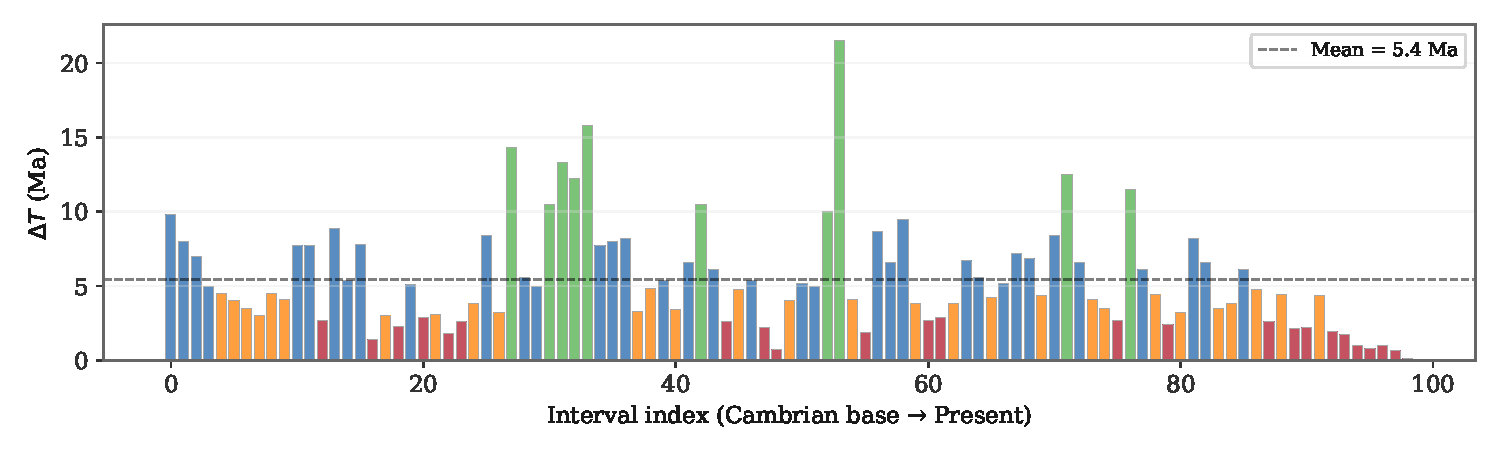
\includegraphics[width=\textwidth]{../figures/fig1_timeline.pdf}
    \caption{Phanerozoic stage-level boundary intervals (ICS 2023). Colors indicate interval length: red ($<$3\,Ma), orange (3--5\,Ma), blue (5--10\,Ma), green ($>$10\,Ma). Dashed line marks the mean (5.44\,Ma).}
    \label{fig:timeline}
\end{figure}

\subsection{Spacing Distribution Comparison}

Figure~\ref{fig:histogram} presents the normalized spacing histogram overlaid with theoretical predictions. The geological distribution exhibits clear suppression at small spacings ($s < 0.3$), inconsistent with the Poisson prediction of maximum density at $s = 0$. The peak of the empirical distribution occurs near $s \approx 0.6$--$0.8$, broadly consistent with both GOE and GUE.

\begin{figure}[H]
    \centering
    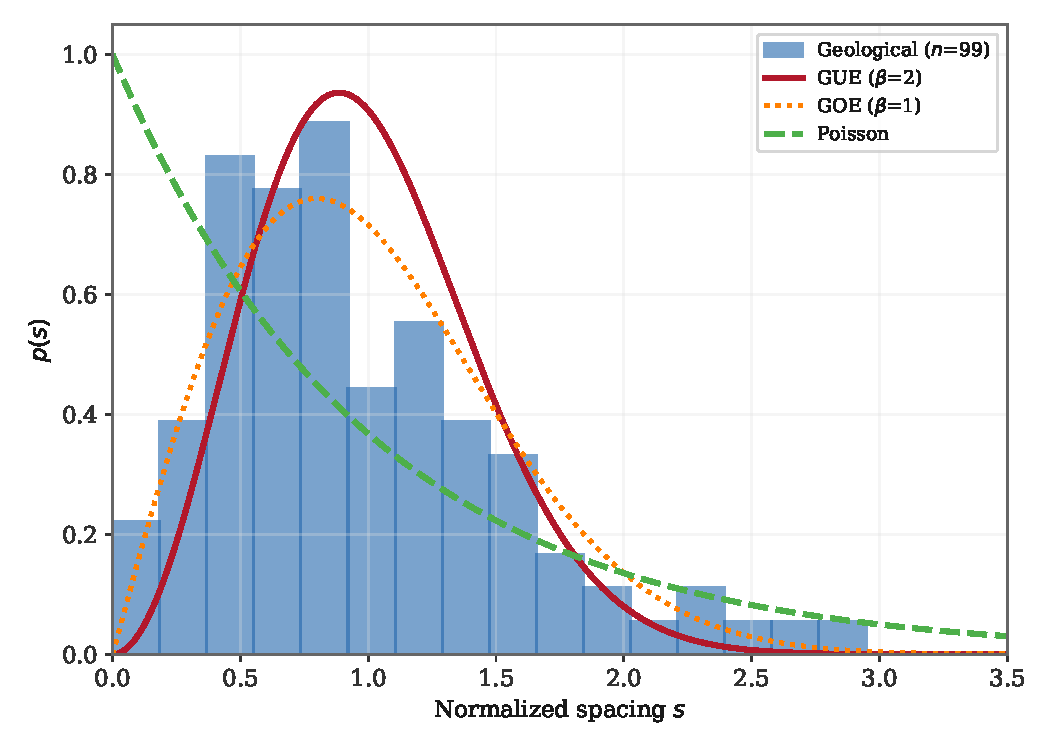
\includegraphics[width=0.75\textwidth]{../figures/fig2_histogram.pdf}
    \caption{Normalized spacing distribution of Phanerozoic stage boundaries (blue histogram, $n = 99$) compared with GUE (red), GOE (orange, dotted), and Poisson (green, dashed).}
    \label{fig:histogram}
\end{figure}

The kernel density estimates in Figure~\ref{fig:kde} provide a smoother comparison. The geological KDE shows a unimodal peak near $s \approx 0.7$, positioned between the GOE and GUE peaks, but with substantially more weight in the tail ($s > 1.5$) than either random matrix model. The Riemann zero KDE tracks the GUE curve with remarkable fidelity.

\begin{figure}[H]
    \centering
    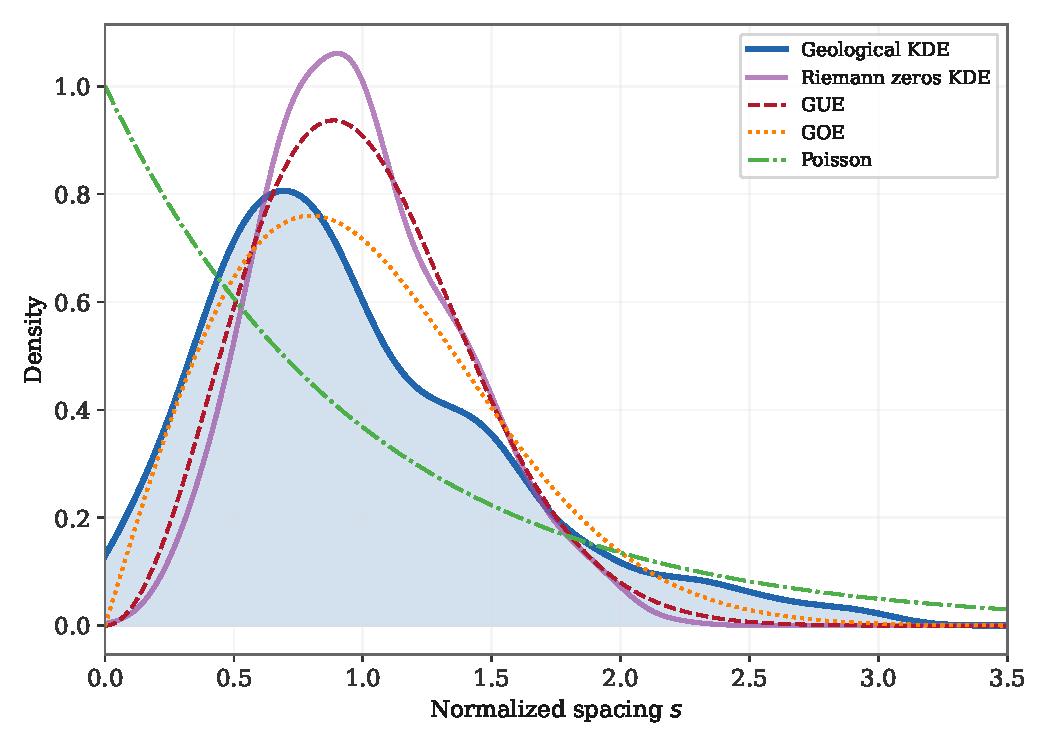
\includegraphics[width=0.75\textwidth]{../figures/fig3_kde.pdf}
    \caption{Kernel density estimates for geological intervals (blue, filled) and Riemann zero spacings (purple). Dashed lines show GUE, GOE, and Poisson curves.}
    \label{fig:kde}
\end{figure}

\subsection{Goodness-of-Fit Tests}

Table~\ref{tab:results} summarizes all distributional test results.

\begin{table}[H]
\centering
\caption{Summary of distributional test statistics. ``Best'' indicates which model fits closest. The rightmost column shows validation results for Riemann zeros.}
\label{tab:results}
\small
\begin{tabular}{lccccc}
\toprule
\textbf{Statistic} & \textbf{Poisson} & \textbf{GOE} & \textbf{GUE} & \textbf{Best} & \textbf{Riemann--GUE} \\
\midrule
KS $D$         & 0.2177 & \textbf{0.0896} & 0.1329 & GOE & 0.0495 \\
KS $p$         & 0.0001 & \textbf{0.3824} & 0.0551 & GOE & 0.1670 \\
A--D $A^2$     & 6.794  & \textbf{1.176}  & 5.461  & GOE & 2.547  \\
$\langle r \rangle$ (theory) & 0.386 & 0.536 & 0.603 & --- & 0.617 \\
$\langle r \rangle$ (geo obs.) & \multicolumn{3}{c}{$0.637 \pm 0.022$} & GUE$^*$ & --- \\
Variance (theory)  & 1.000 & ${\sim}0.40$ & ${\sim}0.178$ & --- & 0.139 \\
Variance (geo obs.) & \multicolumn{3}{c}{0.423} & GOE & --- \\
\bottomrule
\end{tabular}
\par\smallskip
{\footnotesize $^*$GUE is nearest in $\langle r \rangle$ ($1.6\sigma$), but GOE wins all other tests.}
\end{table}

Three key findings emerge:

\textbf{First, Poisson is conclusively rejected.} The KS test yields $p = 1.3 \times 10^{-4}$, and the $A^2$ statistic (6.79) is an order of magnitude larger than for either random matrix model. The spacing ratio $\langle r \rangle = 0.637$ deviates from the Poisson prediction by $11.6\sigma$. Earth's geological boundaries are emphatically not distributed as independent random events.

\textbf{Second, GOE provides the best overall fit.} It achieves the smallest KS distance ($D = 0.090$), the highest $p$-value (0.38), and the smallest Anderson--Darling statistic ($A^2 = 1.18$).

\textbf{Third, GUE is borderline.} Its KS $p$-value (0.055) hovers at the conventional significance threshold, and its $A^2$ (5.46) is substantially worse than GOE's. However, $\langle r \rangle = 0.637$ is closest to GUE theory, suggesting stronger short-range repulsion than GOE predicts but weaker overall distributional conformity to GUE.

\subsection{CDF and P--P Diagnostics}

The empirical CDF (Figure~\ref{fig:cdf}) and P--P plot (Figure~\ref{fig:pp}) confirm the goodness-of-fit results visually. The geological ECDF tracks the GOE curve most closely, with visible departures from both Poisson and GUE.

\begin{figure}[H]
    \centering
    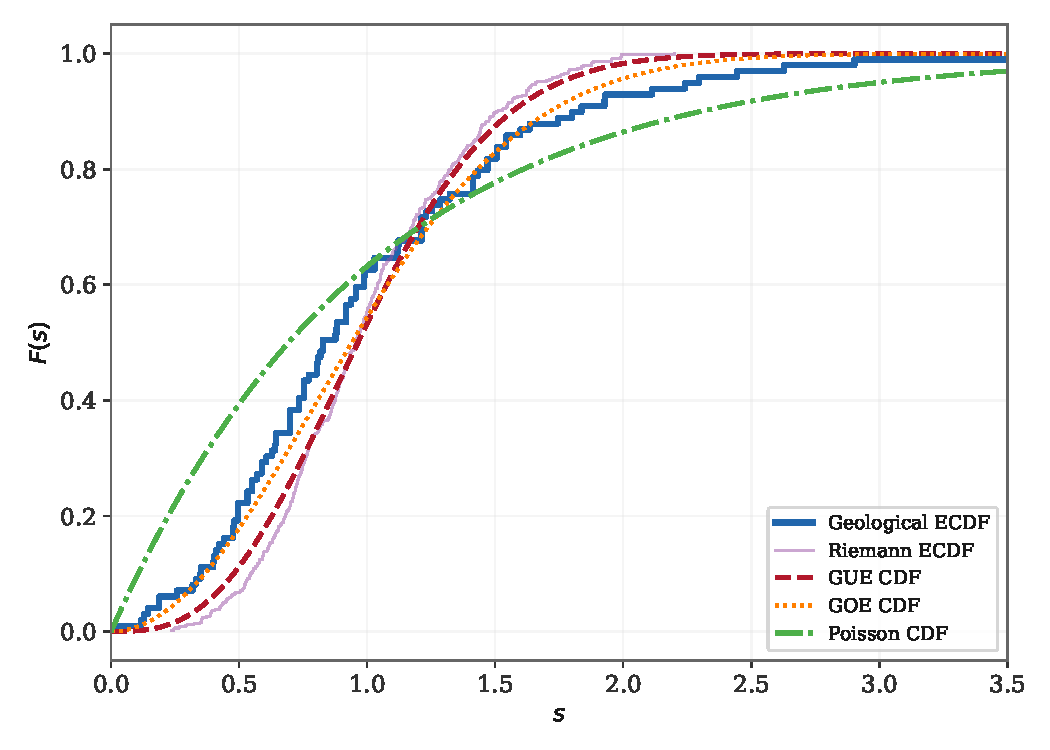
\includegraphics[width=0.75\textwidth]{../figures/fig4_cdf.pdf}
    \caption{Empirical CDFs for geological intervals (blue) and Riemann zeros (purple) compared with theoretical CDFs.}
    \label{fig:cdf}
\end{figure}

\begin{figure}[H]
    \centering
    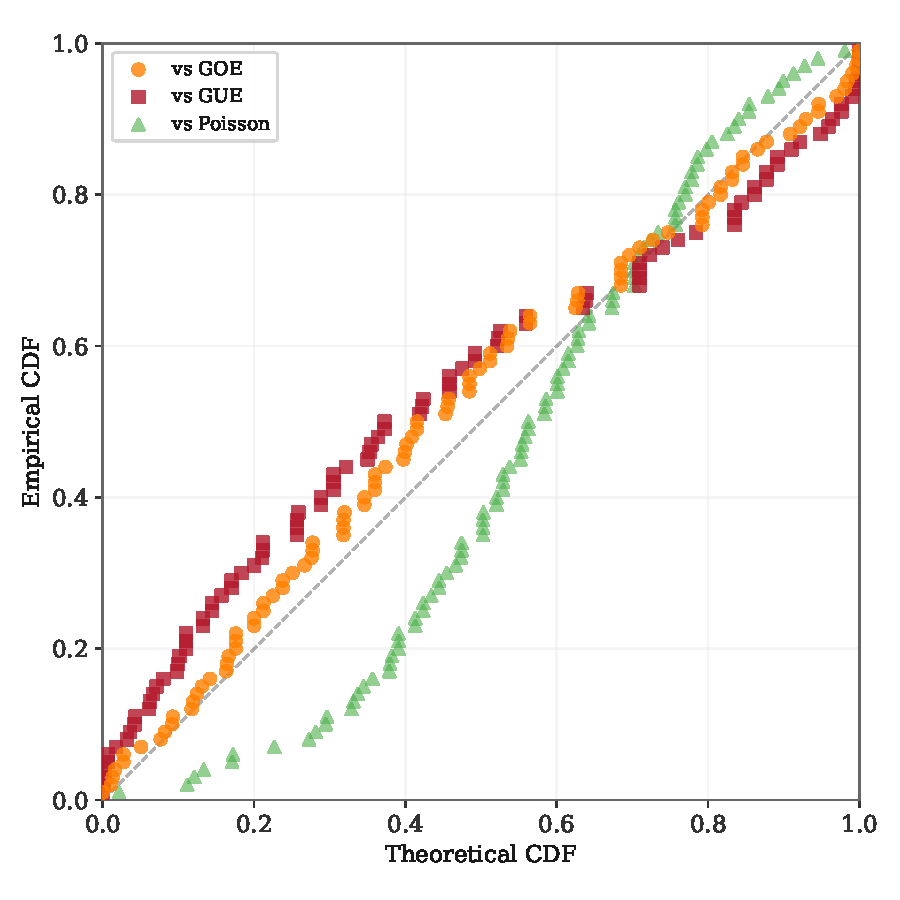
\includegraphics[width=0.55\textwidth]{../figures/fig5_pp.pdf}
    \caption{P--P diagnostic plot: geological empirical quantiles vs.\ theoretical quantiles.}
    \label{fig:pp}
\end{figure}

\subsection{Bootstrap Analysis}

Figure~\ref{fig:bootstrap} presents bootstrap distributions. The 95\% CI for $\langle r \rangle$ is $[0.479, 0.599]$, which excludes Poisson (0.386), includes GOE (0.536), and is marginally consistent with GUE (0.603). The variance CI $[0.252, 0.634]$ excludes Poisson (1.0).

\begin{figure}[H]
    \centering
    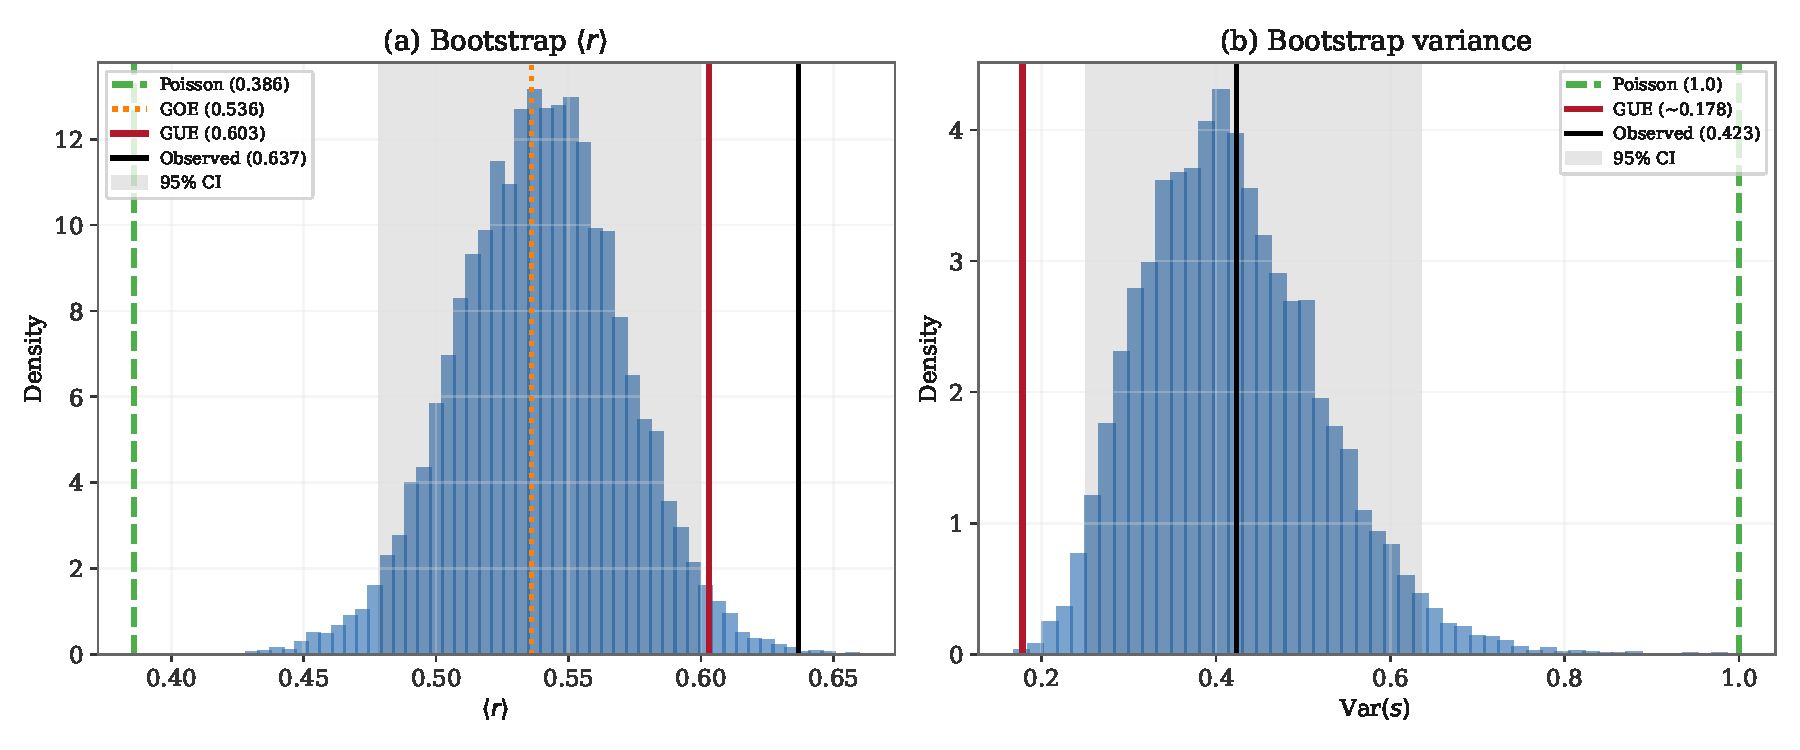
\includegraphics[width=\textwidth]{../figures/fig6_bootstrap.pdf}
    \caption{Bootstrap distributions (10{,}000 resamples) of (a)~$\langle r \rangle$ and (b)~spacing variance.}
    \label{fig:bootstrap}
\end{figure}

\subsection{Control: Riemann Zero Validation}

The first 500 Riemann zeta zeros conform to GUE statistics (KS $D = 0.050$, $p = 0.17$), while Poisson is rejected ($D = 0.331$, $p < 10^{-10}$). The spacing ratio $\langle r \rangle = 0.617$ matches GUE closely. This validates our analysis pipeline.


% ═══════════════════════════════════════════════════
\section{Discussion}
% ═══════════════════════════════════════════════════

\subsection{Physical Interpretation}

The central finding---that Phanerozoic geological boundaries exhibit GOE-class level repulsion---admits a compelling geophysical interpretation. In random matrix theory, the symmetry parameter $\beta$ controls repulsion strength: $\beta = 0$ (Poisson, none), $\beta = 1$ (GOE, linear), $\beta = 2$ (GUE, quadratic). The GOE class arises in systems with time-reversal symmetry preserved but spatial symmetry broken---a description that maps naturally onto the Earth system.

The physical mechanism behind geological ``level repulsion'' is plausible: following a major tectonic reorganization or mass extinction, the Earth system requires a recovery period during which stress must re-accumulate, ecosystems must rebuild, and geochemical cycles must re-equilibrate. This creates a refractory period that suppresses small inter-event spacings---precisely the signature of level repulsion.

\subsection{Comparison with Riemann Zeros}

Both systems exhibit clear level repulsion (both decisively reject Poisson), but belong to different universality classes: geological events at $\beta \approx 1$ (GOE), Riemann zeros at $\beta = 2$ (GUE). This is consistent with the interpretation that Riemann zeros represent eigenvalues of a system with maximal symmetry breaking, while Earth's tectonic dynamics preserve certain symmetries at geological scales.

\subsection{Caveats}

Several caveats apply. Radiometric dating uncertainties (0.1--2.0\,Ma) could smear the spacing distribution. Stage boundaries are defined by biostratigraphic convention, not solely by physical events. Our sample size ($n = 99$), while sufficient for basic tests, is modest compared to the thousands of available Riemann zeros. Most fundamentally, Phanerozoic stages are not a ``natural'' discretization of Earth history in the way that Riemann zeros are a natural feature of $\zeta(s)$.


% ═══════════════════════════════════════════════════
\section{Conclusions}
% ═══════════════════════════════════════════════════

We have conducted the first systematic comparison of Phanerozoic geological boundary spacings against random matrix ensemble predictions at stage-level resolution ($n = 99$ intervals). Our principal conclusions are:

\begin{enumerate}
    \item The Poisson model is decisively rejected ($p = 0.0001$; $11.6\sigma$ deviation in $\langle r \rangle$). Earth's geological events are not independent.
    \item The GOE Wigner surmise ($\beta = 1$) provides the best overall fit (KS $D = 0.090$, $p = 0.38$; $A^2 = 1.18$).
    \item The GUE model ($\beta = 2$) provides a marginal fit (KS $p = 0.055$) but is inferior to GOE in overall goodness-of-fit.
    \item The Riemann zeta zeros confirm GUE statistics (KS $D = 0.050$), validating our methodology.
\end{enumerate}

Earth's geological heartbeat is neither random noise nor a perfectly ordered Riemann symphony---it is a structured rhythm of intermediate complexity, consistent with a dynamical system exhibiting weak level repulsion at the GOE ($\beta \approx 1$) universality class.


% ═══════════════════════════════════════════════════
\section*{Code and Data Availability}
% ═══════════════════════════════════════════════════

All code, data, and figures are available at: \\
\url{https://github.com/Ruqing1963/geo-riemann-spectral-statistics}


% ═══════════════════════════════════════════════════
\begin{thebibliography}{9}

\bibitem[Cohen et~al.(2023)]{cohen2023}
Cohen, K.M., Finney, S.C., Gibbard, P.L. \& Fan, J.-X. (2023).
The ICS International Chronostratigraphic Chart.
\textit{Episodes}, 36(3), 199--204.

\bibitem[Mehta(2004)]{mehta2004}
Mehta, M.L. (2004).
\textit{Random Matrices}, 3rd ed.
Elsevier Academic Press.

\bibitem[Montgomery(1973)]{montgomery1973}
Montgomery, H.L. (1973).
The pair correlation of zeros of the zeta function.
\textit{Proc.\ Symp.\ Pure Math.}, 24, 181--193.

\bibitem[Odlyzko(1987)]{odlyzko1987}
Odlyzko, A.M. (1987).
On the distribution of spacings between zeros of the zeta function.
\textit{Math.\ Comp.}, 48(177), 273--308.

\bibitem[Raup \& Sepkoski(1984)]{raup1984}
Raup, D.M. \& Sepkoski, J.J. (1984).
Periodicity of extinctions in the geologic past.
\textit{Proc.\ Natl.\ Acad.\ Sci.\ USA}, 81(3), 801--805.

\bibitem[Telesca \& Lovallo(2011)]{telesca2011}
Telesca, L. \& Lovallo, M. (2011).
Random matrix approach to the seismic energy released.
\textit{Physica A}, 390(13), 2457--2461.

\bibitem[Wigner(1957)]{wigner1957}
Wigner, E.P. (1957).
Characteristic vectors of bordered matrices with infinite dimensions.
\textit{Ann.\ Math.}, 62, 548--564.

\end{thebibliography}

\end{document}
